%!TEX root=../oi-magistr-spolecne.tex
\section[PAL - Složitost, fronty, haldy]{Amortizovaná složitost. Prioritní fronty, haldy (binární, d-regulární, binomiální, Fibonacciho), operace nad nimi a jejich složitost.}

\paragraph{Amortizovaná složitost.} Amortizovaná časová složitost označuje časovou složitost algoritmu v sekvenci nejhorších možných vstupních dat. Na rozdíl od průměrné složitosti nevyužívá pravděpodobnosti a je proto zaručená \cite{algoritmy:amortizovanaslozitost}.

\textbf{Asymptotická} složitost je \textbf{deklarována na základě nejhorší} (nejlepší) možné \textbf{instance běhu} algoritmu, což \textbf{ale} není vždy vypovídající, protože \textbf{i nejhorší sekvence případů může mít výrazně lepší průběh}, než by asymptotická složitost napovídala. Tento zdánlivý paradox je zapříčiněn tím, že operace s vysokou složitostí změní datovou strukturu tak, že takto špatný případ nenastane po nějakou delší dobu - tím se složitá operace amortizuje.

Jako jednoduchý příklad můžeme uvést specifickou implementaci dynamického pole, která zdvojnásobuje velikost pole pokaždé, když dojde k jeho naplnění. V tomto případě je tedy nutná realokace, v nejhorším případě tato operace potřebuje čas až $O(n)$ - což je asymptotická složitost. Samotné vkládání prvků (bez nutnosti realokace) vyžaduje čas $O(1)$, pro $n$ prvků tedy také $O(n)$. Pro vložení $n$ prvků (včetně realokace) je tedy potřeba $O(n) + O(n) = O(n)$, amortizovaný čas na jedno vložení prvku je pak $O(n)/n = O(1)$ \cite{wiki:amortizovana}.

\paragraph{Definice.} Je dána datová struktura $D$, na které postupně provádíme posloupnost stejných operací. Začneme s $D_0 = D$. První operace zavolaná na $D_0$ upraví datovou strukturu na $D_1$. Druhá operace zavolaná na $D_1$ upraví datovou strukturu na $D_2$. A tak dále. Postupně zavoláme $i$-tou operaci na $D_{i-1}$ a ta upraví datovou strukturu na $D_i$. Některá operace může trvat krátce, jiná déle. Průměrný čas doby trvání operace nazveme amortizovanou časovou složitostí. Amortizovanou časovou složitost jedné operace spočítáme tak, že spočteme celkovou časovou složitost posloupnosti operací v nejhorším případě a vydělíme ji počtem operací.

K čemu je amortizovaná časová složitost? Pomůže nám lépe odhadnout časovou složitost některých algoritmů v nejhorším případě \cite{algoritmyeu:amortizovana}.

\begin{itemize}[itemsep=0pt, topsep=0pt]
    \item Účetní metoda
     \item Metoda potenciálu
\end{itemize}

\noindent Interaktivní struktury: \url{https://www.cs.usfca.edu/~galles/visualization/Algorithms.html}

\subsection{Prioritní fronta \textit{(Priority Queue)}}
Prioritní fronta je \textit{abstraktní datový typ}, podobný klasické frontě či zásobníku s tím rozdílem, že každý element má svou \uv{prioritu}. V prioritní frontě je element s vyšší prioritou vybrán dříve než element s nižší prioritou. Pokud dva elementy mají stejnou prioritu, vyberou se v pořadí v jakém byly vloženy.

\paragraph{Operace.} Prioritní fronta musí implementovat alespoň následující operace:

\begin{itemize}[itemsep=0pt, topsep=2pt]
    \item[-] \texttt{void push(Element e)} - vloží element do prioritní fronty
    \item[-] \texttt{Element pull()} - vybere z fronty element s nejvyšší prioritou
\end{itemize}

\subsection{Haldy}
Halda (minimální) obecně je datová struktura (obvykle stromová) splňující \textbf{vlastnost haldy}:

\begin{center}
    \textit{Pokud B je potomek A, pak B $\geq$ A}
\end{center}

\subsubsection*{Binární halda (Binary heap)}
(Minimální) binární halda je binární strom s dvěma dalšími omezeními:

\begin{enumerate}[itemsep=0pt, topsep=2pt]
    \item Je to kompletní binární strom krom posledního patra (nemusí být úplné). Elementy posledního patra se plní zleva doprava.
    \item Každý element je menší nebo roven vůči jeho potomkům (vlastnost haldy).
\end{enumerate}

\noindent Je to jedna z možných implementací prioritní fronty. Reprezentovat ji můžeme pomocí pole (obr. \ref{fig:heap_array_representation}), kde prvek na indexu (číslováno od 1) $i$ má potomky na indexech $2i$ a $2i + 1$ a rodiče na indexu $i/2$.

\begin{figure}[htbp]
    \begin{center}
        \vspace{-20px}
        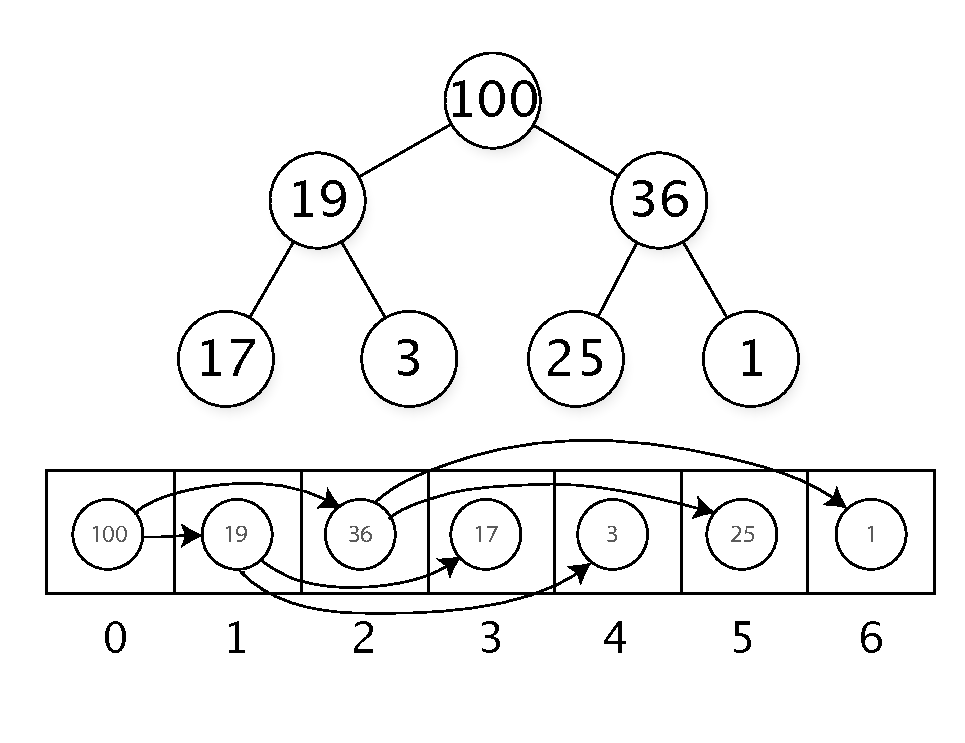
\includegraphics[width=100mm]{01/images/Max-Heap}
        \vspace{-20px}
        \caption{Reprezentace (maximální) binární haldy v poli}
        \label{fig:heap_array_representation}
        \vspace{-20px}
    \end{center}
\end{figure}

\paragraph{Operace.} Operace binární haldy a jejich složitosti:

\begin{itemize}[itemsep=0pt, topsep=2pt]
    \item \texttt{accessMin()} - vrátí hodnotu kořene stromu (typicky první prvek pole)
    \item \texttt{deleteMin(e)} - vrátí element \texttt{e}, který je kořenem stromu, na jeho místo vloží nejpravější prvek \texttt{y} ze spodního patra a poté, pokud je \texttt{y} větší než jeho nejmenší potomek, prohazuji \texttt{y} s jeho nejmenším potomkem do té doby, dokud je \texttt{y} větší než jeho nově vzniknuvší nejmenší potomek,  (tzv. \texttt{y} probublává stromem dolů).
    \item \texttt{insert(e)} - přidáme element \texttt{e} na konec haldy a dokud je předek větší než \texttt{e}, tak je prohazujeme (probublávání směrem nahoru).
    \item \texttt{delete(e)} - podobně jako \texttt{deleteMin()}, odeberu element \texttt{e} a nechám ho probublat
    \item \texttt{merge(h1, h2)} - sloučí 2 haldy, vytvoří nové pole, kam nakopíruje obsah obou hald a na toto nové pole zavolá proceduru \texttt{heapify()}. Ta jede od půlky pole směrem na začátek (navštíví všechny podhaldy) a každý vrchol podhaldy nechá probublat a správně zařadit.
    \item \texttt{decreaseKey(k, v)} - zmenšíme hodnotu elementu s klíčem \texttt{k} o \texttt{v} a necháme probublat stromem.
\end{itemize}

\begin{table}[ht]
    \centering
    \vspace{0px}
    \begin{tabu}{|[1pt]c|c|c|[1pt]}
        \tabucline[1pt]{-}
        operace & čas. složitost & poznámka \\\tabucline[1pt]{-}
        \texttt{accessMin()} & $\Theta (1)$ &  \textcolor{gray}{přístup k vrcholu haldy} \\\hline
        \texttt{deleteMin()} & $\Theta (\log(n))$ &  \textcolor{gray}{smazání vrcholu haldy} \\\hline
        \texttt{insert(e)} & $\Theta (\log(n))$ &  \textcolor{gray}{přidání prvku do haldy} \\\hline
        \texttt{delete(e)} & $\Theta (\log(n))$ &  \textcolor{gray}{smazání elementu haldy} \\\hline
        \texttt{merge(h1,h2)} & $\Theta (n_1 + n_2)$ &  \textcolor{gray}{sloučení 2 hald} \\\hline
        \texttt{decreaseKey(k,v)} & $\Theta (\log(n))$ &  \textcolor{gray}{snížení hodnoty klíče $k$ o $v$} \\\hline
    \end{tabu}
    \caption{Binární halda - Operace a jejich složitosti}
\label{table:bin_heap_complexity}
\end{table}

\subsubsection{D-regulární halda (D-ary heap)}
D-regulární halda je zobecnění binární haldy, kde počet potomků se rovná číslu $d$, namísto 2 jako je tomu v haldě binární. $d$ nám udává počet štěpení stromu haldy. Operace jsou identické jako v binární haldě. Časová složitost operací je téměř stejná, liší se jen v základu logaritmu (u binární haldy je základ 2, tady $d$). Pro efektivní implementaci je vhodné zvolit $d$ jako mocninu 2. V tomto případě lze totiž využít bitových posunů - změna indexu při průchodu polem. D-halda běží rychleji než binární pokud velikost haldy převyšuje velikost cache počítače \cite{pal:prednasky}.

\paragraph{Operace.} Operace d-regulární haldy a jejich složitosti:
\begin{table}[ht]
    \centering
    \vspace{0px}
    \begin{tabu}{|[1pt]c|c|c|[1pt]}
        \tabucline[1pt]{-}
        operace & čas. složitost & poznámka \\\tabucline[1pt]{-}
        \texttt{accessMin()} & $\Theta (1)$ &  \textcolor{gray}{přístup k vrcholu haldy} \\\hline
        \texttt{deleteMin()} & $\Theta (\log_d(n))$ &  \textcolor{gray}{smazání vrcholu haldy} \\\hline
        \texttt{insert(e)} & $\Theta (\log_d(n))$ &  \textcolor{gray}{přidání prvku do haldy} \\\hline
        \texttt{delete(e)} & $\Theta (\log_d(n))$ &  \textcolor{gray}{smazání elementu haldy} \\\hline
        \texttt{merge(h1,h2)} & $\Theta (n_1 + n_2)$ &  \textcolor{gray}{sloučení 2 hald} \\\hline
        \texttt{decreaseKey(k,v)} & $\Theta (\log_d(n))$ &  \textcolor{gray}{snížení hodnoty klíče $k$ o $v$} \\\hline
    \end{tabu}
    \caption{D-regulární halda - Operace a jejich složitosti}
\label{table:d_heap_complexity}
\end{table}

\subsubsection{Binomiální halda (Binomial heap)}
Binomiální halda je kolekce binomiálních stromů stupňů $i = 0 \hdots \lfloor \log(n) \rfloor$. Každý řád je zastoupen maximálně 1 stromem.

\paragraph{Binomiální strom} je definovám rekurzivně:

\begin{itemize}[itemsep=0pt, topsep=2pt]
    \item Binomiální strom řádu 0 obsahuje jediný prvek - kořen
    \item Binomiální strom řádu $k$ má kořenový element, jehož potomci jsou kořeny binomiálních stromů stupňů $k-1, k-2, \hdots, 2, 1, 0$ (v tomto pořadí)
\end{itemize}

\begin{wrapfigure}{r}{0.55\textwidth}
    \vspace{-20px}
    \begin{center}
        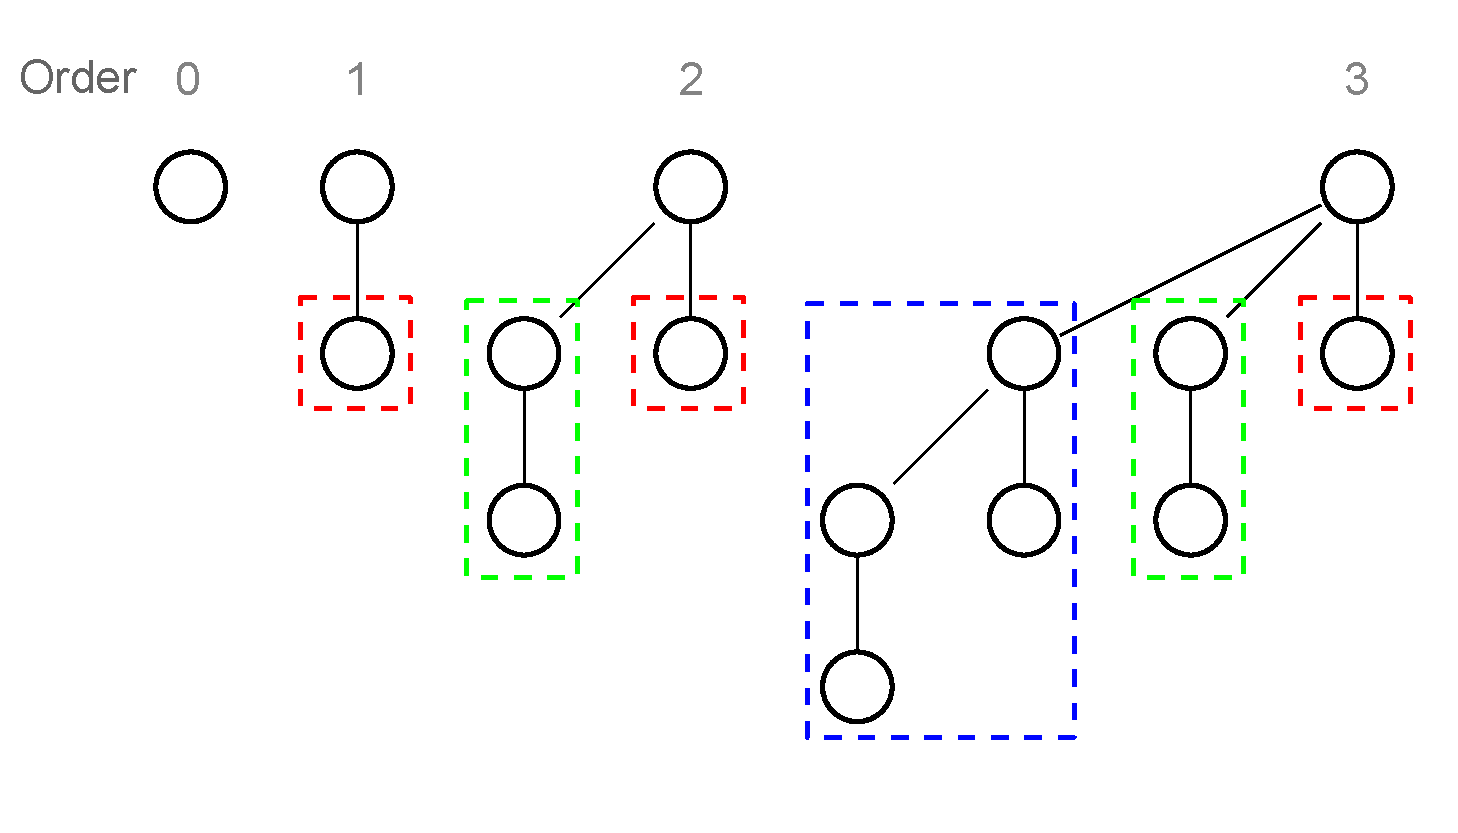
\includegraphics[width=65mm]{01/images/Binomial_Trees}
    \end{center}
    \vspace{-30pt}
    \label{fig:binom_heap}
    \vspace{-60pt}
\end{wrapfigure}

\noindent Pro binomiální strom řádu $k$ platí:

\begin{itemize}[itemsep=0pt, topsep=2pt]
    \item splňuje vlastnost haldy
    \item hloubka stromu je $k$
    \item kořen má $k$ potomků
    \item obsahuje $2^k$ prvků
\end{itemize}

\paragraph{Operace.} Operace binomiální haldy a jejich složitosti:

\begin{itemize}[itemsep=0pt, topsep=2pt]
    \item \texttt{accessMin()} - vrátí kořen binomiálního stromu z MIN ukazatele.
    \item \texttt{deleteMin(e)} - vezmou se všechny podstromy, které vznikly odebráním kořene a ty se postupně mergují s ostatními stromy
    \item \texttt{insert(e)} - z vkládaného prvku se vytvoři nová binomiální halda (strom řádu 0) a ta se merguje s původní haldou
    \item \texttt{delete(e)} - sníží se hodnota pomocí \texttt{decreaseKey} na $-\infty$ a provede se \texttt{deleteMin()}
    \item \texttt{merge(h1, h2)} - Analogie mezi mergeováním dvou hald a binárním sčítáním. Naskládáme si stromy obou hald pod sebe (podle jejich stupňů). Pokud v jedné haldě je strom $i$-tého řádu a v druhé není, tak ho jen opíši. Pokud v obou haldách existují stromy stejného řadu, pak vzniká přenos do vyššího řádu. Kdykoliv vznikne přenos, mergujeme tyto dva stromy do sebe. Díky struktuře stromů, se provádí merge, porovnáním jejich kořenů, menší z kořenů se stane kořenem nově vzniklého stromu (řádu o 1 vyšší) a druhý strom se stane jeho potomkem.
    \item \texttt{decreaseKey(k, v)} - podobné jako u binární haldy
\end{itemize}

\begin{figure}[htbp]
    \begin{center}
        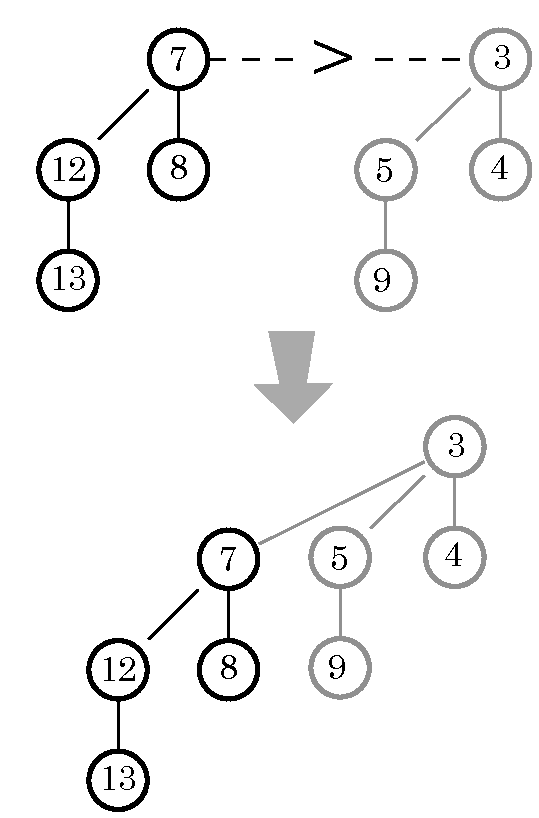
\includegraphics[width=45mm]{01/images/Binomial_heap_merge1}
        \hspace{50px}
        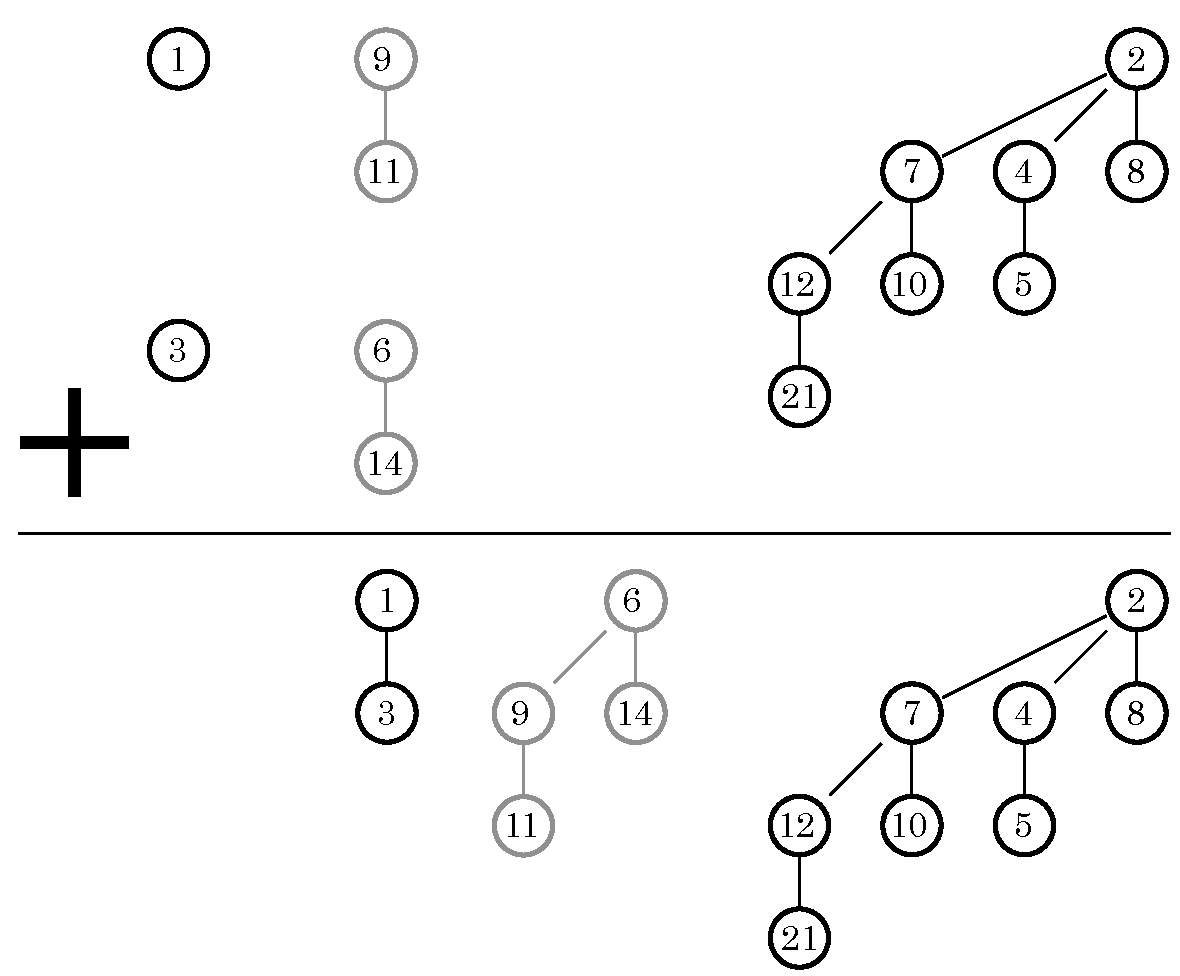
\includegraphics[width=85mm]{01/images/Binomial_heap_merge2}
        \caption{Binomiální halda MERGE - 2 příklady}
        \label{fig:binom_heap_add}
    \end{center}
\end{figure}

\begin{table}[ht]
    \centering
    \vspace{0px}
    \begin{tabu}{|[1pt]c|c|c|[1pt]}
        \tabucline[1pt]{-}
        operace & čas. složitost & poznámka \\\tabucline[1pt]{-}
        \texttt{accessMin()} & $\Theta (1)$ &  \textcolor{gray}{přístup k vrcholu haldy} \\\hline
        \texttt{deleteMin()} & $\Theta (\log(n))$ &  \textcolor{gray}{smazání vrcholu haldy} \\\hline
        \texttt{insert(e)} & $\Theta (\log(n))$ amortizovaně: $\Theta(1)$ &  \textcolor{gray}{přidání prvku do haldy} \\\hline
        \texttt{delete(e)} & $\Theta (\log(n))$ &  \textcolor{gray}{smazání elementu haldy} \\\hline
        \texttt{merge(h1,h2)} & $\Theta (\log(n))$ &  \textcolor{gray}{sloučení 2 hald} \\\hline
        \texttt{decreaseKey(k,v)} & $\Theta (\log(n))$ &  \textcolor{gray}{snížení hodnoty klíče $k$ o $v$} \\\hline
    \end{tabu}
    \caption{Binomiální halda - Operace a jejich složitosti}
\label{table:binom_heap_complexity}
\end{table}
\vspace{-10px}
\subsubsection{Fibonacciho halda}
Založena na binomiální haldě. Má relaxovanější strukturu, která umožňuje zlepšené asymptotické složitosti. Fibonacciho halda se nevyužívá v real-time systémech, protože některé operace mají lineární složitost. U operací, které nevyžadují mazání (accesMin, merge, decreaseKey) je amortizovaná složitost $O(1)$.

\paragraph{Struktura.} Fibonacciho haldu tvoří skupina stromů vyhovující lokální podmínce na uspořádání haldy, která vyžaduje, aby pro každý uzel stromu platilo, že prvek, který reprezentuje, je menší než prvek reprezentovaný jeho potomky. Z této podmínky vyplývá, že minimálním prvkem je vždy kořen jednoho ze stromů. Vnitřní struktura Fibonacciho haldy je v porovnání s binomiální haldou daleko více flexibilní. Jednotlivé stromy nemají pevně daný tvar a v extrémním případě může každý prvek haldy tvořit izolovaný strom nebo naopak všechny prvky mohou být součástí jediného stromu hloubky $n$. Tato flexibilní struktura umožňuje velmi jednoduchou implementaci operací s haldou. Operace, které nejsou potřebné, odkládáme a vykonáváme je až v okamžiku, kdy je to nevyhnutelné, například spojení nebo vložení nového prvku se jednoduše provede spojením kořenových seznamů (s konstantní náročností) a jednotlivé stromy spojíme až při operaci snížení hodnoty klíče \cite{wiki:fibonacci}.

\paragraph{Implementace.} Pro rychlé vymazání a zřetězení se vytváří \textit{obousměrný cyklický spojový seznam} kořenů všech stromů (obr. \ref{fig:fibonacci_heap}). Pro potomky každého prvku se vytváří podobný seznam. Pro každý uzel se ukládá počet synů a údaj, zda je zvýrazněn. Navíc si uchováváme ukazatel na kořenový prvek s minimální hodnotou klíče ($MIN$) \cite{wiki:fibonacci}.

\begin{figure}[htbp]
    \begin{center}
        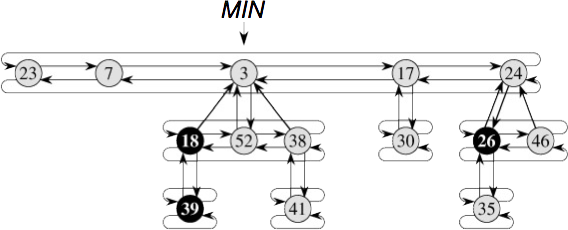
\includegraphics[width=140mm]{01/images/fibonacci_heap}
        \caption{Reprezentace fibonacciho haldy}
        \label{fig:fibonacci_heap}
    \end{center}
\end{figure}

\begin{itemize}[itemsep=0px]
\item \textbf{N} - aktuální počet prvků
\item \textbf{MIN} - minimum haldy
\item \textbf{rank} - pomocné pole pří slévání stromů (označení stupně stromů)
\item \textbf{mark(x)} - boolean hodnota indikující jestli prvek x ztratil potomka od té doby kdy x bylo vytvořeno jako potomek jiného prvku. Nově vytvořené prvky jsou neoznačené, a prvek x se stane neoznačeným, vždy když se stane potomkem jiného prvku.
\end{itemize}

\paragraph{Operace.} Operace Fibonacciho haldy a jejich složitosti:

\begin{itemize}[itemsep=0pt, topsep=2pt]
    \item \texttt{accessMin()} - vrátí kořen z Fibonacciho stromu na který ukazuje $MIN$ pointer
    \item \texttt{deleteMin()} - Operace odstranění minima probíhá ve třech krocích. V prvním odstraníme kořenový prvek s minimální hodnotou klíče. Jeho synové vytvoří kořenové prvky nových stromů. Poté se slévají stromy stejného stupně, a nakonec se upraví ukazatel MIN. Při slévání stromů tvořících jednu haldu postupně sjednotíme kořeny stromů stejných stupňů. Uvažujeme, že počet kořenových prvků na počátku operace je N. Pokud máme dva kořeny U a V stejného stupně, vytvoříme z jednoho z nich syna druhého prvku tak, aby kořenovým zůstal prvek s menší hodnotou klíče. Jeho stupeň se pak zvětší o jedničku. Toto opakujeme, dokud v haldě existují dva stromy se stejným stupněm. K efektivnímu hledání stromů stejného stupně používáme pole ukazatelů, ve kterém uchováváme reference vždy na jeden kořen každého stupně. Pokud je nalezen druhý strom stejného stupně, oba stromy jsou spojeny a příslušný ukazatel v poli je aktualizován
    \item \texttt{insert(e)} - vytvoří se nová halda obsahující jediný element \texttt{e}; \texttt{mark(e) = false}; Merge s původní haldou - $O(1)$
    \item \texttt{merge(h1, h2)} - prosté spojení seznamů s kořenovými prvky stromů jednotlivých hald a update $MIN$ pointeru
\end{itemize}

\begin{table}[ht]
    \centering
    \vspace{0px}
    \begin{tabu}{|[1pt]c|c|c|[1pt]}
        \tabucline[1pt]{-}
        operace & čas. složitost & poznámka \\\tabucline[1pt]{-}
        \texttt{accessMin()} & $O(1)$ &  \textcolor{gray}{přístup k vrcholu haldy} \\\hline
        \texttt{deleteMin(e)} & $O(n)$ amortizovaně: $O(\log(n))$ &  \textcolor{gray}{smazání vrcholu haldy} \\\hline
        \texttt{insert(e)} & $O(1)$ &  \textcolor{gray}{přidání prvku do haldy} \\\hline
        \texttt{delete(e)} & $O(n)$ amortizovaně: $O(\log(n))$ &  \textcolor{gray}{smazání elementu haldy} \\\hline
        \texttt{merge(h1,h2)} & $O(1)$ &  \textcolor{gray}{sloučení 2 hald} \\\hline
        \texttt{decreaseKey(k,v)} & $O(\log(n))$ amortizovaně $O(1)$ &  \textcolor{gray}{snížení hodnoty klíče $k$ o $v$} \\\hline
    \end{tabu}
    \caption{Fibonacciho halda - Operace a jejich složitosti}
\label{table:fibo_heap_complexity}
\end{table}

\paragraph{\texttt{deleteMin()}} Popis operace \texttt{deleteMin} a následné konzolidace haldy.

\lstset{style=php,caption=deleteMin ve Fibonacciho haldě, label=listing:fib_delete}
\begin{lstlisting}[mathescape]
z = MIN;
if (z $\neq$ null) then {
  foreach x $\in$ descendants(z) do
    add $x$ to the root list of the heap;
  remove $z$ from the root list of the heap;
  if (N=1) then {
    MIN = null;
  } else {
    MIN = any pointer to a root from the root list of the heap;
    Consolidate();
  }
  N--;
}
\end{lstlisting}

\lstset{style=php,caption=Konzolidace ve Fibonacciho haldě, label=listing:fib_consol}
\begin{lstlisting}[mathescape]for i = 0 to max. possible degree of a tree in Fibo. heap of size N do A[i] = null;
foreach w $\in$ all trees in the root list of the heap do {
  x = w; d = a degree of the tree w;
  while rank[d] $\neq$ null do {
    y = rank[d];
    if key(x) > key(y) then swap x and y;
    remove y from the root list of the Heap;
    make y a child of x, incrementing the degree of x;
    mark(y) = false; rank[d] = null; d++;
  } 
  rank[d] = x;
}
MIN = null;
for i = 0 to max. degree of a tree in the array A do {
  if rank[i] $\neq$ null then {
    add rank[i] to the root list of the heap;
    If (MIN = null) or (key(A[i]) < key(MIN)) then MIN = A[i];
  }
}
\end{lstlisting}

\begin{table}[ht]
    \centering
    \vspace{0px}
    \begin{tabu}{|[1pt]c|c|c|c|c|[1pt]}
        \tabucline[1pt]{-}
        & \textbf{binary heap} & \textbf{d-ary heap} & \textbf{binomial heap} & \textbf{Fibonacci heap} \\\tabucline[1pt]{-}
         \texttt{accessMin()} & $\Theta (1)$ &  $\Theta (1)$ & $\Theta (1)$ & $\Theta (1)$ \\\hline
        \texttt{deleteMin()} & $\Theta (\log(n))$ & $\Theta (\log(n))$ & $\Theta (\log(n))$ & $O(n);O(\log(n))$ \\\hline
        \texttt{insert(e)} & $\Theta (\log(n))$ & $\Theta (\log(n))$ & $O(\log(n));O(1)$ & $\Theta (1)$ \\\hline
        \texttt{delete(e)} & $\Theta (\log(n))$ & $\Theta (\log(n))$ & $O(\log(n))$ & $O(n); O(\log(n))$ \\\hline
        \texttt{merge(h1,h2)} & $\Theta (n)$ & $\Theta (n)$ & $O (\log(n))$ & $\Theta (1)$ \\\hline
        \texttt{decreaseKey(k,v)} & $\Theta (\log(n))$ & $\Theta (\log(n))$ & $\Theta (\log(n))$ & $O(\log(n)); O(1)$ \\
        \hline
    \end{tabu}
    \caption{Haldy - srovnání složitostí}
\label{table:heaps_complexities}
\end{table}

% https://www.cs.princeton.edu/~wayne/teaching/fibonacci-heap.pdf

\begin{figure}[htbp]
    \begin{center}
        \vspace{-20px}
        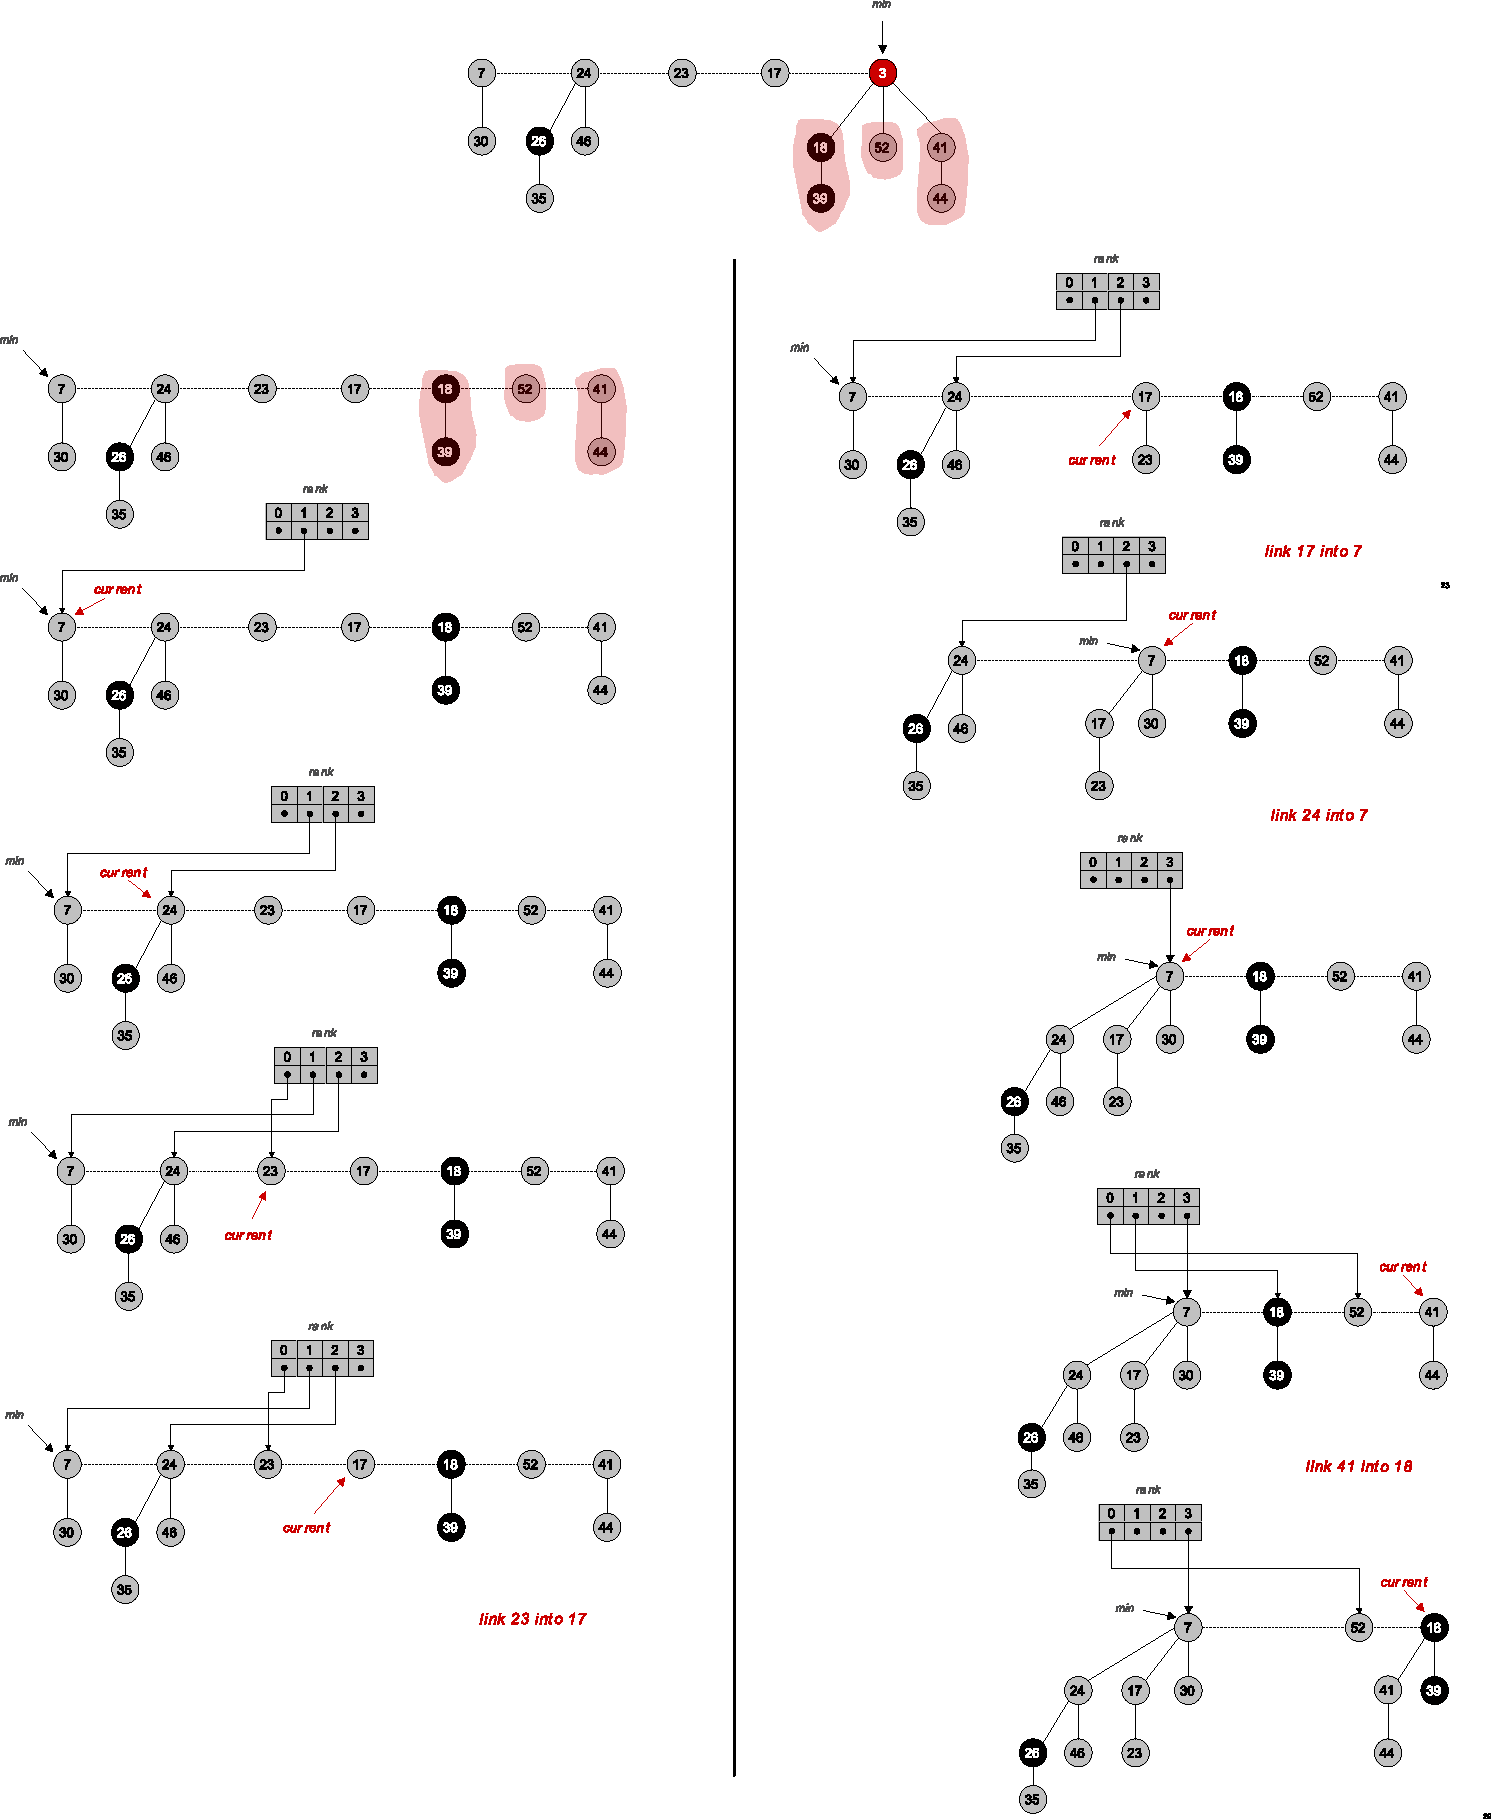
\includegraphics[width=160mm]{01/images/fib-heap-del}
        \caption{Postup při deleleMin operaci}
        \label{fig:bin-heap-del}
    \end{center}
\end{figure}
